\subsection{RAID 01}

RAID 0+1 (RAID 01) es un RAID compuesto que combina striping (RAID 0) y mirroring (RAID 1).

Conceptualmente, primero se crean dos o más arreglos RAID 0, distribuyendo los datos entre los discos para obtener un alto rendimiento. Luego, esos arreglos RAID 0 se duplican mediante RAID 1, de modo que uno es el espejo del otro.

\begin{figure}[!ht]
  \centering
  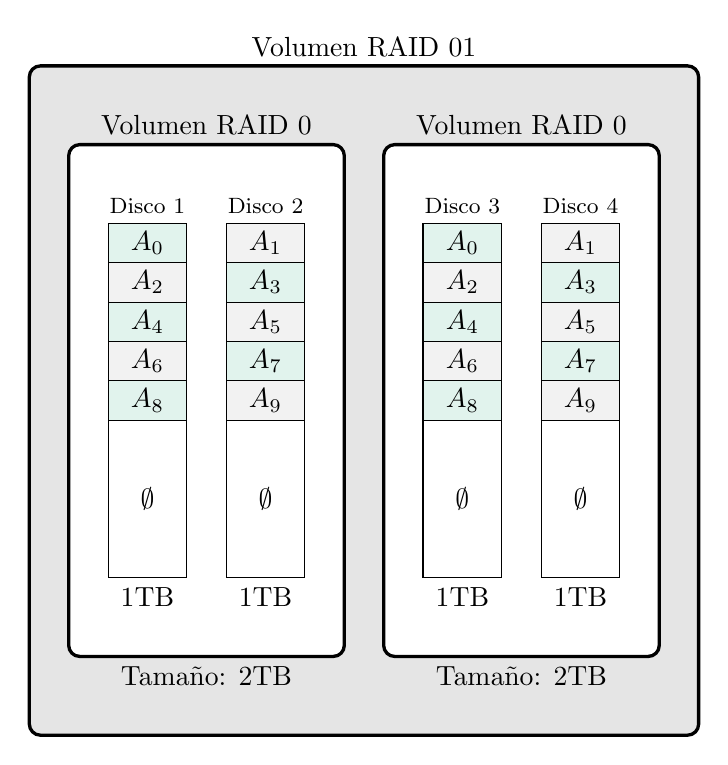
\begin{tikzpicture}
    % RAID 1 

    \draw[very thick,rounded corners,fill=gray!20] (-1,-4) rectangle (7.5,4.5);
    \node[above] at (3.25,4.5) {Volumen RAID 01};

    % caja RAID 0 arreglo 1
    \draw[very thick,rounded corners,fill=white] (-0.5,-3) rectangle (3,3.5);
    \node[above] at (1.25,3.5) {Volumen RAID 0};
    \node[below] at (1.25,-3) {Tamaño: 2TB};

    % caja RAID 0 arreglo 2
    \draw[very thick,rounded corners,fill=white] (3.5,-3) rectangle (7,3.5);
    \node[above] at (5.25,3.5) {Volumen RAID 0};
    \node[below] at (5.25,-3) {Tamaño: 2TB};

    % Primer arreglo de RAID 0

    \node[above,font=\footnotesize] at (0.5,2.5) {Disco 1};
    \foreach \y\t\c in {
        0/8/white!95!blue!93!green,
        0.5/6/gray!10,
        1/4/white!95!blue!93!green,
        1.5/2/gray!10,
        2/0/white!95!blue!93!green}{
      \draw[fill=\c] (0,\y) rectangle node{\(A_\t\)} (1,{0.5+\y});
    }
    \draw (0,0) rectangle node{\(\emptyset\)} (1,-2);
    \node[below] at (0.5,-2) {1TB};

    \node[above,font=\footnotesize] at (2,2.5) {Disco 2};
    \foreach \y\t\c in {
        0/9/gray!10,
        0.5/7/white!95!blue!93!green,
        1/5/gray!10,
        1.5/3/white!95!blue!93!green,
        2/1/gray!10}{
      \draw[fill=\c] (1.5,\y) rectangle node{\(A_\t\)} (2.5,{0.5+\y});
    }
    \draw (1.5,0) rectangle node{\(\emptyset\)} (2.5,-2);
    \node[below] at (2,-2) {1TB};

    % Segundo arreglo de RAID 0

    \node[above,font=\footnotesize] at (4.5,2.5) {Disco 3};
    \foreach \y\t\c in {
        0/8/white!95!blue!93!green,
        0.5/6/gray!10,
        1/4/white!95!blue!93!green,
        1.5/2/gray!10,
        2/0/white!95!blue!93!green}{
      \draw[fill=\c] (4,\y) rectangle node{\(A_\t\)} (5,{0.5+\y});
    }
    \draw (4,0) rectangle node{\(\emptyset\)} (5,-2);
    \node[below] at (4.5,-2) {1TB};

    \node[above,font=\footnotesize] at (6,2.5) {Disco 4};
    \foreach \y\t\c in {
        0/9/gray!10,
        0.5/7/white!95!blue!93!green,
        1/5/gray!10,
        1.5/3/white!95!blue!93!green,
        2/1/gray!10}{
      \draw[fill=\c] (5.5,\y) rectangle node{\(A_\t\)} (6.5,{0.5+\y});
    }
    \draw (5.5,0) rectangle node{\(\emptyset\)} (6.5,-2);
    \node[below] at (6,-2) {1TB};
  \end{tikzpicture}
  \caption{Tamaño del volumen de RAID 01: 2TB.}
  \label{fig:raid01}
\end{figure}

Por ejemplo, un arreglo RAID 01 con cuatro discos tendría una configuración como la representada en la figura \ref{fig:raid01}.

Cuando se escribe un dato:
\begin{enumerate}
  \item Se distribuye entre los discos del primer RAID 0.
  \item Esa misma distribución se copia íntegramente al segundo RAID 0.
\end{enumerate}

\paragraph{Características}
\begin{itemize}
  \item Combina el alto rendimiento de RAID 0 con la redundancia de RAID 1.
  \item Requiere al menos cuatro discos.
  \item La capacidad útil es el 50\% de la capacidad total, ya que una mitad del almacenamiento se destina al espejo.
\end{itemize}

\paragraph{Tolerancia a fallos}
RAID 01 puede soportar la falla de un disco, ya que el otro RAID 0 contiene una copia completa de los datos.

Sin embargo, si falla un disco de uno de los arreglos RAID 0, ese arreglo completo deja de ser funcional y el sistema pasa a depender únicamente del otro espejo. A partir de ese momento, cualquier falla adicional en el arreglo restante implica la pérdida de los datos.

Por ello, aunque RAID 01 ofrece redundancia, su tolerancia a múltiples fallos es inferior a la de RAID 10, motivo por el cual este último suele preferirse en implementaciones modernas.

\begin{table}[!ht]
  \centering
  \begin{tabular}{l|c}
    Cantidad de discos mínima & 4 \\\hline
    Cantidad de discos que pueden fallar & 1 \\ \hline
    Velocidad de escritura relativa a un disco & \(N/2\times\)VDisco~[MB/s] \\\hline
    Velocidad de escritura ponderada & 10 \\ \hline
    Velocidad de lectura relativa a un disco & \(N/2\times\)VDisco~[MB/s] \\ \hline
    Velocidad de lectura ponderada & 10 \\ \hline
    Costo & Alto
  \end{tabular}
  \caption{Características del RAID 01.}
\end{table}
